\chapter{Initialisierung}

\label{ReportInitialisierung}

\section{Ausgangslage}

\section{Projektziele}

\begin{longtable}[]{@{}lll@{}}
  \toprule
  Nr.  & Zielbeschreibung                                                                       & Muss/Kann\tabularnewline
  \toprule
       & Produktziele\tabularnewline
  \midrule
  1.1  & Besucher können im Produkt nach Konzerten suchen                                       & Muss\tabularnewline
  1.2  & Suchresultate können nach Musik-Genre und Ort gefiltert werden                         & Muss\tabularnewline
  1.3  & Das Produkt soll ein modernes responsives Design vorweisen                             & Muss\tabularnewline
  1.4  & Konzerte sollen von Suchmaschinen indexiert werden können                              & Muss\tabularnewline
  1.5  & Benutzer können isch im Produkt registrieren                                           & Muss\tabularnewline
  1.6  & Benutzer können ihr Passwort nach Verlust neu setzen                                   & Muss\tabularnewline
  1.7  & Inhalte des Portals sind durch die Benutzer erfassbar und bearbeitbar                  & Muss\tabularnewline
  1.8  & Kompatibilität mit aktuellem Google Chrome und Mozilla Firefox Browser                 & Muss\tabularnewline
  1.9  & Konzerte können vom Produkt nach Facebook exportiert werden                            & Kann\tabularnewline
  1.10 & Ein angemeldeter Benutzer kann vermerken ob er einem Konzert teilnimmt                 & Kann\tabularnewline
  1.11 & Das Produkt soll sich an Security Best-Practices von OWASP halten                      & Muss\tabularnewline
  \bottomrule
       & Abwicklungsziele\tabularnewline
  \midrule
  2.1  & \makecell[l]{Das Projekt soll nach HERMES 5 unter Berücksichtigung der Richtlinien von                            \\ der TSBE dokumentiert werden} & Muss\tabularnewline
  2.2  & Das Produkt muss bis Projektende fertiggestellt und bereit für die Einführung sein     & Muss\tabularnewline
  2.3  & Die Technische-Umsetzung wird durch Damian Senn erstellt                               & Muss\tabularnewline
  2.4  & \makecell[l]{Die Kommunikation zwischen Experten und Diplomanden erfolgt wie im                                   \\ Projektauftrag \ref{kommunikation} beschrieben.} & Muss\tabularnewline
  2.5  & Das Projekt muss bis Ende Mai 2019 abgeschlossen sein                                  & Muss\tabularnewline
  \bottomrule
\end{longtable}


\clearpage

\section{Projektorganisation}

\begin{figure}[!htb]
  \centering
  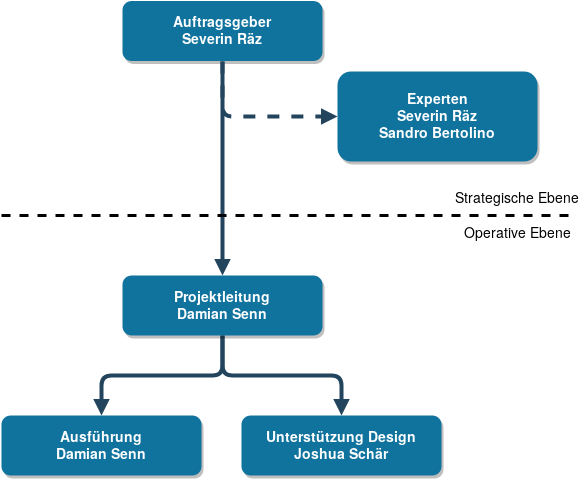
\includegraphics[width=0.8\textwidth]{figures/organigram.png}
  \caption{Organigram}
\end{figure}

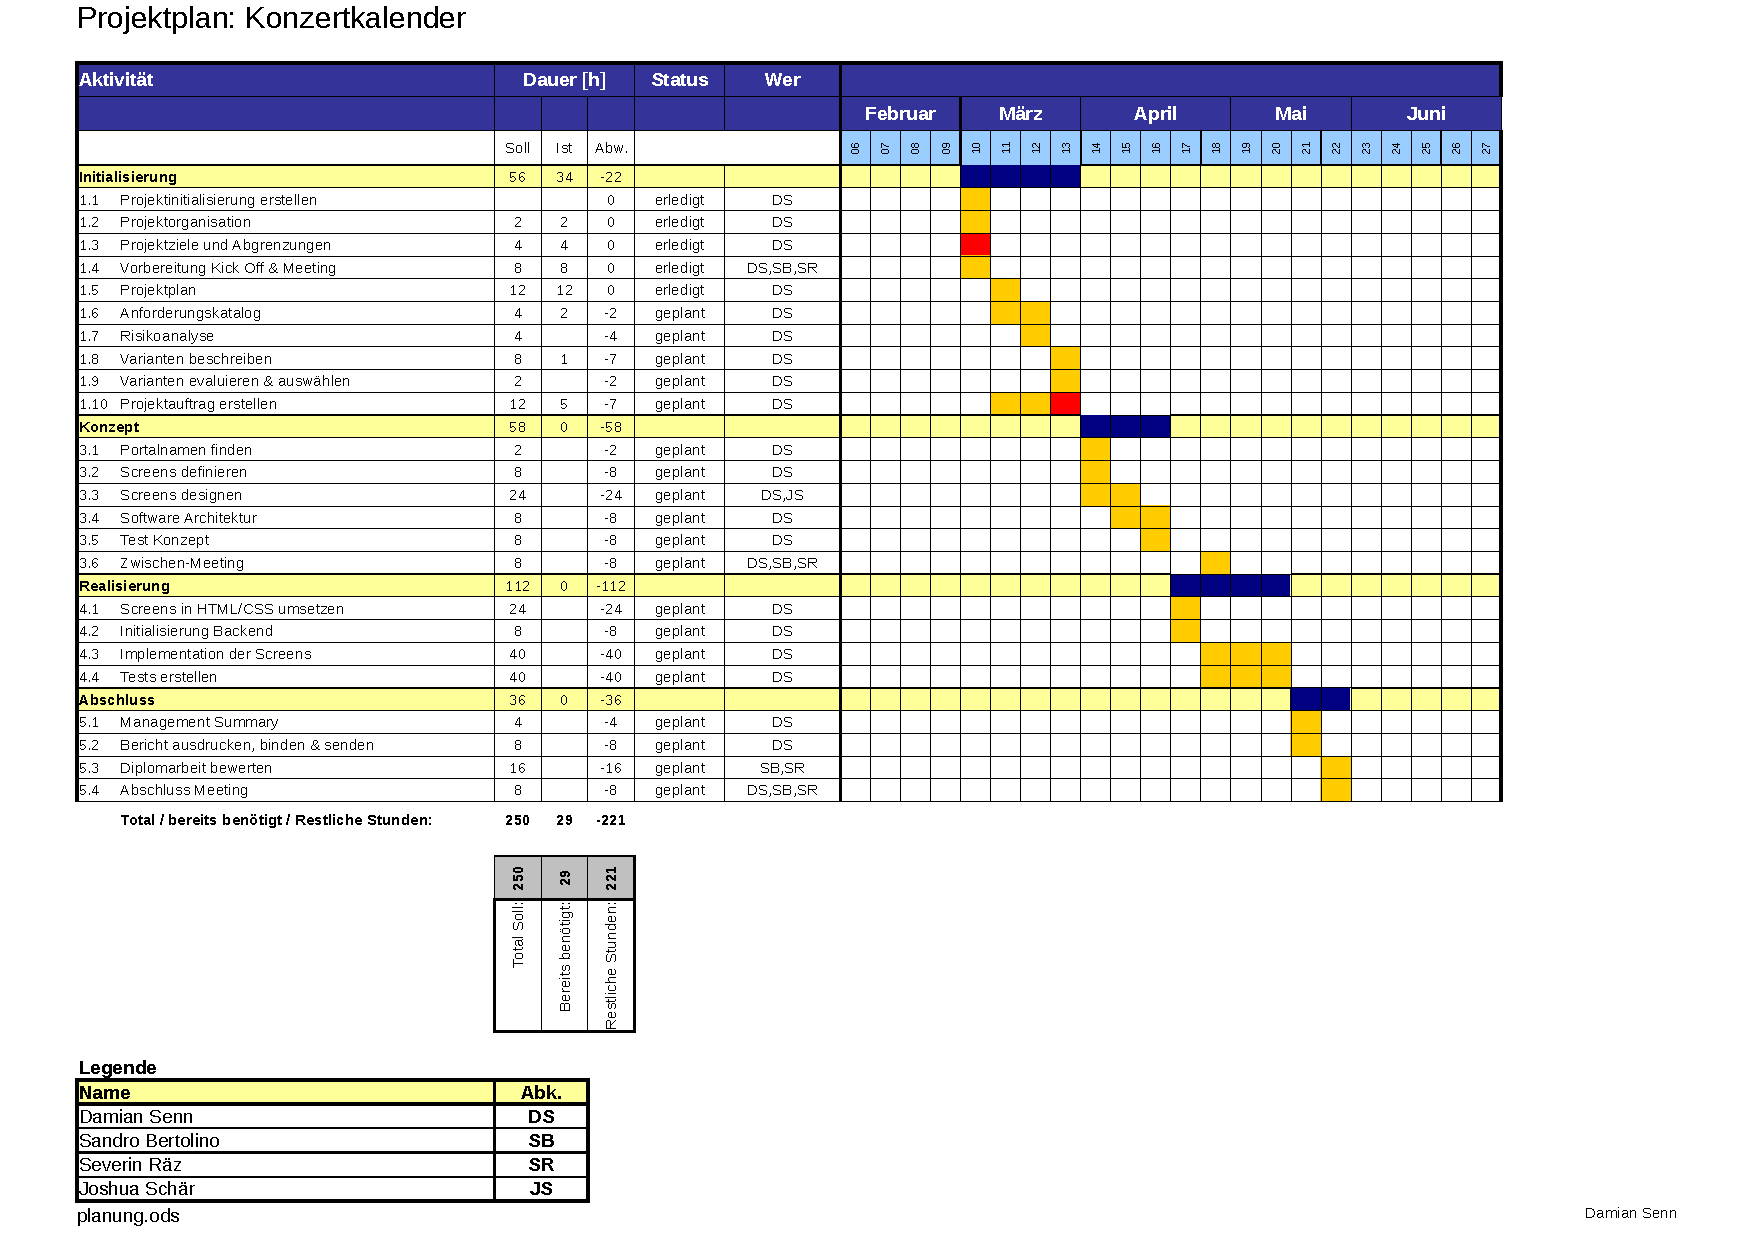
\includepdf[pagecommand={\section{Ausgefüllter Projektplan}}]{initialisierung/planung.pdf}

\section{Lieferergebnisse}

\section{Ressourcenplan}

\section{Risiken}

\clearpage

\section{Abgrenzungen}

\begin{figure}[!htb]
  \centering
  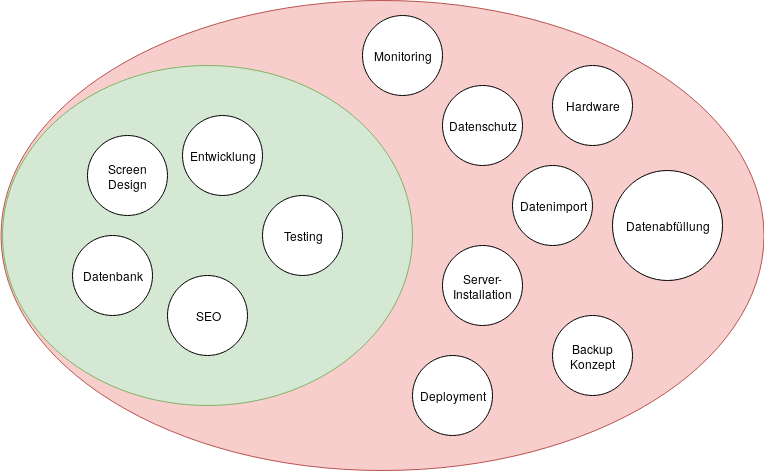
\includegraphics[width=0.95\textwidth]{figures/abgrenzungen.png}
  \caption{Abgrenzungen}
\end{figure}

Die detaillierten Erklärung zu den Abgrenzungen sind im Projektauftrag~\ref{abgrenzungen} zu finden.

\clearpage

\section{Studie}

\subsection{Informationsbeschaffung}

\subsection{Anforderungskatalog}

\subsection{Pflichtenheft}

\subsection{Mögliche Varianten}

\subsection{Evaluation Varianten}

\subsection{Entscheid Varianten}

\subsection{Wirtschaftlichkeit}
